% \chapter{DESIGN STEPS FOR SEAMLESS BRIDGE SYSTEM DEVELOPED BY SHRP 2 R19A}
\chapter{SHRP2 R19A开发的无缝桥接系统设计步骤}
Expansion joints are one of the main causes for high maintenance costs in bridges. A new seamless bridge system was envisioned within the SHRP 2 R19A project that should result in bridges with long service lives by eliminating the joints over the entire length of the bridge, approach slab, and a segment of the roadway (Ala and Azizinamini 2013a; Ala and Azizinamini 2013b). The system is similar to a system developed in Australia for use with continuously reinforced concrete pavements (CRCP) (Bridge et al. 2000). Proposed modifications have been made to the Australian system to adapt it to United States practice in which most pavements are either jointed plain concrete or flexible pavement (Ala 2011). While pavement within a particular roadway may be jointed or flexible, the segment of roadway containing the bridge and the proposed seamless transition is similar in nature to CRCP. Therefore, transition details would be similar to those used when transitioning from CRCP to jointed or flexible pavements.

The key factor is establishing an effective longitudinal force transfer mechanism from the transition slab to the base soil that minimizes the length of the transition. The goal is achieving limited end movements, a predictable and controlled crack pattern, and controlled axial forces in the system.

The system that was developed to meet these needs is shown in \cref{fig:bridge-roadway-interface}. The transition slab is connected to a secondary slab that is embedded below. The two slabs are connected by a series of small piles. The secondary slab increases the stiffness of the transition region resulting in the desired short transition length. A similar system without the transition slab may lose its effectiveness after multiple cycles due to compaction of the soil surrounding the small piles.


\begin{figure}
  % \includegraphics[width=\linewidth]{graphic-file}
  % \caption{Schematic and rendering of the recommended practice for bridge/roadway interface.}
  \caption{桥梁/道路界面推荐做法}
  \label{fig:bridge-roadway-interface}
\end{figure}

A special reinforcement reduction detail is used over the length of the transition zone to achieve a controlled crack pattern when the bridge system is in tension. The system behavior in tension (temperature reduction/bridge contraction) is an important factor since the crack pattern plays a major role in design life and maintenance costs. \cref{fig:gradual-transition} shows a transition in which the reinforcement detail helps to maintain the desirable crack pattern (Jung et al. 2007). The reinforcement is reduced over the length of the transition region as the force is reduced.

\begin{figure}
  % \includegraphics[width=\linewidth]{graphic-file}
  % \caption{Gradual transition continuously reinforced to jointed pavement. (Jung et al. 2007)}
  \caption{台后到接缝路面的逐步过渡与加固}
  \label{fig:gradual-transition}
\end{figure}

Analysis, design, and construction of a seamless bridge and approach slab system are similar to other bridge structures. However, there are some new components involved in the system that are not typically seen in other bridge systems. The new components include transition slab, secondary slab, small piles, and the connection of the small piles to the transition concrete slabs. \cref{fig:small-piles-connect-slabs} shows an example of the small piles used to connect the transition slab to the secondary slab during the developmental phase of the concept.

\begin{figure}
  % \includegraphics{small-piles-connect-slabs1.pdf}
  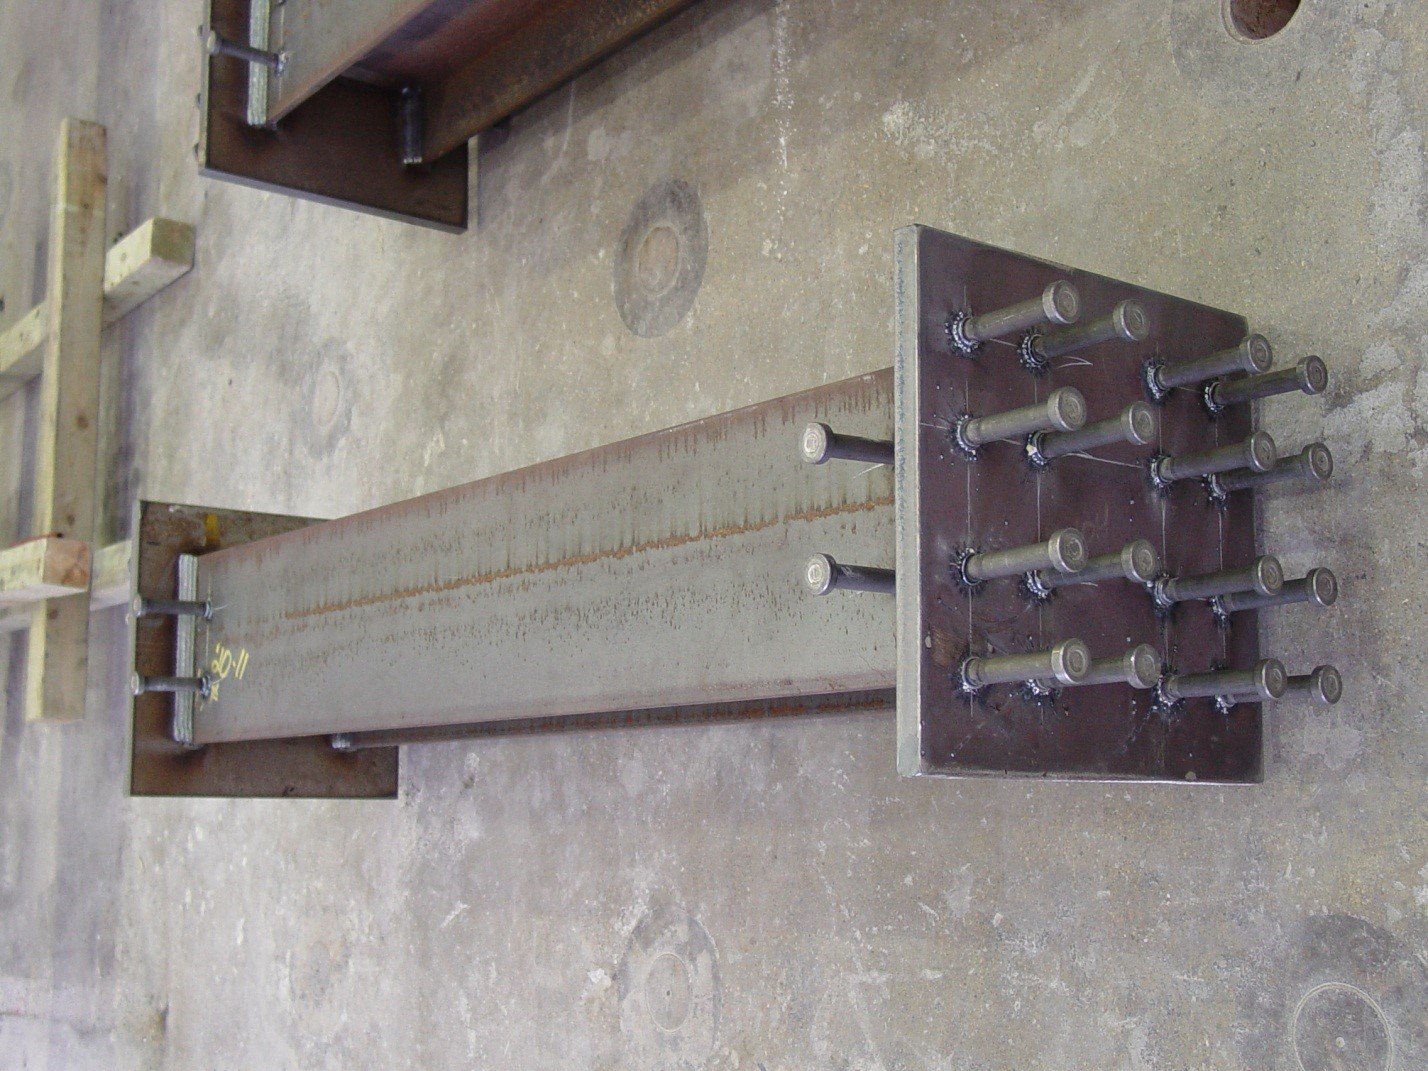
\includegraphics[width=0.7\linewidth]{small-piles-connect-slabs2.jpg}
  % \caption{Small piles to be used in the test to connect the upper and lower slabs.}
  \caption{试验中用小桩连接上下板}
  \label{fig:small-piles-connect-slabs}
\end{figure}

The initial system design is an iterative process in which the length of the transition and secondary slabs; the shape, size, and spacing of small piles; and the embedment depth of the secondary slab are determined via structural analyses of various system configurations. Demand in all components is determined during the initial design phase. The various parts of the system may then be designed according to the applicable AASHTO LRFD Bridge Design Specifications (LRFD Specifications). The reduced cracked stiffness of the system in tension may be neglected in the initial design.

Relevant pavement design loadings are the longitudinal strains (thermal effects, creep, and shrinkage) and the out-of-plane effects (due to traffic wheel loads, settlement of approach embankments, and rotational effects transferred from the bridge deck).

% \section{STRUCTURAL ANALYSIS}
\section{结构分析}
Until further research is completed to develop a simplified analysis approach, the seamless bridge should be analyzed as a holistic system with all components incorporated in the analysis. To account for the effect of temperature changes in design of the transition region of the seamless bridge system, only the effect of uniform temperature change needs to be considered. The calculation of uniform temperature change should be in accordance with LRFD Specifications Article 3.12.2. The interaction between the soil and the small piles can be modeled in the structural analysis using springs. The spring stiffness around the small piles highly depends on the relative density of the compacted soil material (geomaterial) surrounding the small piles and the confinement pressure. Since the soil material is manually compacted, the relative density of the compacted soil needs to be measured during the compaction process and this compaction should be related to the soil stiffness. The connection of the small piles to the slabs can be assumed rigid for analysis purposes.

The structural analysis should take into account the effects of longitudinal stiffness reduction due to cracking of the transition slab in tension (temperature reduction/bridge contraction). Iterative structural analyses of the seamless bridge and roadway system in conjunction with cracked section analyses are required. For the first iteration, the tensile forces in the structure are assumed equal to the compressive forces due to thermal expansion. Cracked section analyses are carried out for various segments of the transition slab, and the axial stiffness of the slab segments are modified. The structure is analyzed with the modified in-plane stiffness to determine the in-plane tensile axial forces in the system. This process is repeated until convergence of the axial forces is achieved.

% \section{DESIGN OF THE SYSTEM COMPONENTS}
\section{\glsentrytext{system}\glsentrytext{component}设计}
Once the initial system design has been completed, design of the individual system components can be performed.

% \subsection{Approach Slab and Bridge Deck}
\subsection{引板和桥面板}
Extra reinforcement may be required in the approach slab for crack control under the tensile in-plane forces due to thermal expansion. The bridge deck also has to be checked for cracking. The approach slab should be checked for the compressive thermal stresses to avoid concrete crushing. The approach slab should be designed for the differential settlement of the bridge abutment and the transition system. Embankment settlement is another important criterion to check for the approach slab. The bridge approach embankments should be designed to achieve a long-term settlement of less than 3/4 in. to minimize traffic comfort issues on the motorway pavement. To account for the probable geotechnical and construction variations, however, a more conservative approach embankment settlement of 1.5 in. should be assumed for the seamless pavement design (Thomas Telford Service Ltd. 1993).

% \subsection{Transition Slab}
\subsection{Transition Slab}
The main objective of providing a transition slab is to provide a means for controlling the movement of the system to the point in which no expansion devices are needed where the transition slab meets the pavement. The design items for transition slab include designing against compressive force created by thermal expansion; achieving a uniform cracking pattern in the transition zone during contraction, preventing punching shear failure at the pile to slab connection area; and ensuring adequate flexural capacity at these locations. The thickness of the transition slab should be determined based on 
\begin{enumerate*}
  \item the punching shear requirements, 
  \item connection requirements for developing themoment introduced from the small piles, and 
  \item the in-plane horizontal stiffness of the system to reduce themovement of the end joint. 
\end{enumerate*}
Reinforcement of the transition slab should be determined from cracked section analysis under tensile in-plane forces. The transition slab should be checked for the maximum bending moments between the rows of small piles. Stirrups (tie bars) may be required for the connection to the slab around the ends of the small piles. The transition slab should also be designed for the design truck axle load exerted at the midspan of the slab between the small piles. Both slabs should be designed for punching shear and one-way shear. Detailed design provisions are provided in VTrans (2009) and also Ala and Azizinamini (2013a).

% \subsection{Secondary Slab}
\subsection{Secondary Slab}
The length of the secondary slab should be greater than or equal to the length of the transition slab. Likewise, the secondary slab thickness is designed for punching shear and requirements to develop the moment introduced from the small piles into the slab (the secondary slab thickness will most likely be equal to the transition slab). The secondary slab should also be designed for the bending moment due to the soil pressure underneath. This slab should be designed for punching and one-way shear.


% \subsection{Small Piles}
\subsection{Small Piles}
The stiffness, number, and arrangement of small piles connecting the transition and secondary slabs should be determined to control the longitudinal movement of the transition slab at the end where it meets the pavement. This limit eliminates expansion joint devices at these locations. Increasing the stiffness of the small piles will reduce the longitudinal movement of the transition slab at the end of transition zone. However, piles with high flexural stiffness will also create high stresses (tension or compression) in the transition slab and bridge deck, in addition to the secondary slab. Therefore, the design of small piles should consider a balance between longitudinal movement at the end of transition slab, and maximum longitudinal force that can be accommodated in the transition slab and bridge deck. Further, small piles with high stiffness will demand more sophisticated connection details to the transition and secondary slabs. The maximum longitudinal movement at the end of the transition slab, where it meets pavement, should be limited to about 0.25 in.

% \subsection{Connection of Small Piles to the Slabs}
\subsection{Connection of Small Piles to the Slabs}
The connection design for attaching the small piles to the top (transition) and bottom (secondary) slabs should use high factors of safety and ensure that they stay elastic, when the weak element of the entire system fails. This is similar to the philosophy used in seismic design where some of the bridge elements are protected and remain elastic while plastic hinges form in other parts of the structure. The connection should be designed for cyclic loading, as the system will be subjected to daily and seasonal temperature fluctuation. \cref{fig:pile-slab-connection} shows one possible connection detail that was used during the experimental phase. Based on the experimental results, the area around the connection could have a larger thickness or alternatively could use advanced materials such as ultra-high performance concrete (UHPC). Research is needed to develop more economical connection details.

\begin{figure}
  % \includegraphics[width=\linewidth]{graphic-file}
  % \caption{Recommended small pile concrete slab connection.}
  \caption{推荐小桩混凝土板连接}
  \label{fig:pile-slab-connection}
\end{figure}

% \subsection{Geomaterial}
\subsection{Geomaterial}

Design of the geomaterial consists of the selection of the geomaterial type and the compaction requirement. The required compaction depends on the stiffness requirement around the small piles. It is very important to achieve the required compaction (level and consistency) around the small piles so stringent quality control is required during soil compaction. It is highly recommended to use granular material in this region due to ease of compaction, resulting in smaller long-term settlement and smaller gap development around the piles caused by pile movements.

Moisture density relation (compaction) tests, maximum and minimum density (relative density) tests, and in-place moisture content and density determinations during placement of the backfill (using a nuclear moisture density meter) are the recommended soil mechanics tests.

% \section{CRACKED SECTION ANALYSIS}
\section{开裂截面分析}
Methods of determining the maximum probable crack width and stiffness reduction for an axially tensioned concrete member are explained in ACI Report 224.2R-92 (1997). The maximum probable crack width in a fully cracked member can be determined from;
\begin{equation}
  \label{eq:maximum-crack}
  W_\text{max} =0.10\times 10^{-3} f_\text{s} \sqrt[3]{d_\text{c} A}
\end{equation}
\begin{EqDesc}{f_\text{s}}
  \item [d_\text{c}] distance from center of bar to extreme tension fiber (in.),
  \item [f_\text{s}] service stress in the reinforcement (ksi)
  \item [A] effective tension area of concrete surrounding the tension reinforcement, having the same centroid as the reinforcement, divided by the number of bars (sq.in.)
\end{EqDesc}

\cref{fig:effective-tension-area} demonstrates the calculation of $A$. $S$ is the bar spacing and $H$ is the total thickness of the slab.

\begin{figure}
  % \includegraphics[width=\linewidth]{graphic-file}
  % \caption{Determination of effective tension area of concrete surrounding the tension reinforcement for an axially tensioned concrete member.}
  \caption{轴向受拉混凝土构件受拉钢筋周围混凝土有效受拉面积的确定}
  \label{fig:effective-tension-area}
\end{figure}

As can be seen in \cref{fig:effective-tension-area}, the parameter $\sqrt[3]{d_\text{c} A}$ can be determined to be $d_\text{c}\sqrt[3]{2S/d_\text{c}}$
for both one and two layers of reinforcement.

The crack width allowed is inserted in \cref{eq:maximum-crack} to obtain the service stress/strain in the reinforcement.

The LRFD Specifications define an exposure factor ($\gamma_\text{e}$) which is 1.00 for Class 1 exposure condition and 0.75 for Class 2 exposure condition. The crack width associated with Class 1 and 2 exposure conditions are 0.017 and 0.012 respectively.

The amount of required reinforcing steel can be determined from the axial tensile force ($P$) in the member (determined from the structural analysis).

\begin{equation}
  P = f_\text{s} A_\text{s} \Rightarrow  A_\text{s} = \frac{P}{f_\text{s}}
\end{equation}
\begin{EqDesc}{A}
  \item[A] reinforcement steel area
\end{EqDesc}

The axial force in various segments of the transition slab (P) is determined from structural analysis. The transition slab may crack when it is in tension. Cracking in the transition slab will result in reduction of axial stiffness. The reduced axial stiffness of the cracked transition slab should be used in structural analysis, requiring an iterative cracked section analysis. In this iterative analysis the section axial stiffness is modified based on the axial force determined from the previous analysis. Next, the structure is analyzed using the modified axial stiffness. This process is repeated until convergence. For the first iteration, the slab can be assumed un-cracked (the tensile force can be taken the same as the compressive force developed in the slab due to temperature increase).

Following is a description of the method for determining the reduced axial stiffness of the concrete member in tension.

The ACI Report 224.2R-92 (1997) suggests the following equation for determining the direct tensile strength of the concrete ($f'_\text{t}$).
\begin{equation}
  f'_\text{t} = 0.33\left[ \gamma_\text{c} f'_\text{c}\right]^{\frac12}
\end{equation}
Where: From the LRFD Specifications, for a given $f'_\text{c}$, the unit weight can be determined from $\gamma_\text{c} = 0.14 + 0.001f'_\text{c}$ and
the $E_\text{c}$ can be determined from $E_\text{c}=33000K_1\gamma_c^{1.5}\sqrt{f'_\text{c}}$

The stress in the reinforcing bars after the crack occurs ($f'_\text{s,cr}$) is determined from ACI Report 224.2R-92 (1997).
\begin{equation}
  f'_\text{s,cr} = f'_\text{t} \left( \frac{1}{\rho} -1 +n \right)
\end{equation}
\begin{EqDesc}{\rho}
  \item [\rho] 配筋率($A_\text{s}/A_\text{g}$);
  \item [n] 钢筋与混凝土的弹性模量比。
\end{EqDesc}

The axial load that causes first cracking in the axially tensioned member is;
\begin{equation}
  P_\text{cr} = f'_\text{s,cr} \times A_\text{s}
\end{equation}

During the cracked section analysis, if the force in a segment of the slab is smaller than $P_\text{cr}$ , the slab will not crack and no modification will be required in the structural analysis. Otherwise, if the force in a segment of the transition slab exceeds the above $P_\text{cr}$ , the segment will crack and the modified axial stiffness of the segment should be determined and used for the next iteration.

For a cracked section, the average strain in the tensile member can be calculated from the CEB Model Code (Thomas Telford Service Ltd. 1993) using following equation to determine the modified axial stiffness;
\begin{equation}
  \varepsilon_\text{m}=\varepsilon_\text{s}\left[ 1-k \left( \frac{f_\text{s,cr}}{f_\text{s}}\right)^2 \right]
\end{equation}
In which $\varepsilon_\text{s}=f_\text{s}/E_\text{s}$, $k = 1.0$ for first loading and 0.5 for repeated or sustained loading. $k=0.5$ should be used
for the seamless system.

The following equation provides the effective modulus of elasticity of steel bars;
\begin{equation}
  E_\text{sm} = \frac{E_\text{s}}{\left[1- 1-k \left( \dfrac{f_\text{s,cr}}{f_\text{s}}\right)^2 \right]}
\end{equation}

The effective axial cross-sectional stiffness of the tensile concrete member can be written as $(EA)_\text{eff}= E_\text{sm} A_\text{s}$. The ratio term $(EA)_\text{eff}/(EA)$ is the section modification factor that should be used in the structural analysis to modify the axial stiffness of the member in tension. \cref{fig:cracked-section-analysis} shows the general flowchart for the cracked section analysis.

\begin{figure}
  % \includegraphics[width=\linewidth]{graphic-file}
  % \caption{Cracked section analysis flowchart}
  \caption{开裂截面分析流程}
  \label{fig:cracked-section-analysis}
\end{figure}